\documentclass[11pt]{article}
\usepackage{arxiv}
\usepackage{xurl}
\usepackage{tikz}
\usetikzlibrary{positioning,arrows.meta,fit}
\usepackage{tabularx}
\setlength{\emergencystretch}{2em}
% Generated from the frozen evidence by reproduction/scripts/analyze.py.
\newcommand{\LongTokens}{21549}
\newcommand{\LongSeconds}{371.9}
\newcommand{\LongPhaseRate}{57.95}
\newcommand{\LongSumRate}{70.24}
\newcommand{\LongTTFT}{50.52}
\newcommand{\CounterMedian}{70.67}
\newcommand{\CounterMean}{45.86}
\newcommand{\HeadRegression}{2.71}
\newcommand{\InflightRegression}{4.60}
\newcommand{\MTPFleet}{66.81}
\newcommand{\MTPDeployment}{64.36}
\newcommand{\EvidenceFiles}{421}
\newcommand{\ExperimentCount}{50}
\newcommand{\PhaseCount}{160}
\newcommand{\TelemetryCount}{35}

\newcommand{\expid}[1]{\texttt{#1}}
\title{A 975B Mixture-of-Experts Model on Eleven AI PCs:\\Memory, Scheduling, and Numerical Limits of Integrated-GPU Inference}
\author{
Tate Berenbaum\\Community Labs\\\texttt{tb@communitylabs.com}
\and Matias Parij\\Community Labs\\\texttt{mparij@communitylabs.com}
\and Muthaiah Venkatachalam\\Intel Corporation\\\texttt{muthaiah.venkatachalam@intel.com}
}
\date{September 2026}
\begin{document}
\maketitle

\begin{abstract}
Can a fleet of client machines serve a nearly trillion-parameter mixture-of-experts model, and which constraints remain once its weights fit? We study Cascadia running the text path of Inkling, a 975B-total/41B-active-parameter model, across eleven Intel Core Ultra X7 358H systems with 64\,GB of nominal memory each and gigabit Ethernet. Six consecutive decoder layers reside on each machine; integrated GPUs execute compressed projections and fused expert operations while CPUs maintain attention and sequence state. A 176-request run generates \LongTokens{} tokens in \LongSeconds{} seconds: \LongPhaseRate{} tokens/s including admission, compared with \LongSumRate{} tokens/s when summing individual decode rates. At fifteen concurrent requests, eight-row prefill windows reduce observed median first-token latency from 31.2--31.5\,s to 6.91\,s. The study documents memory-residency failures caused by fallback execution, a dense-to-fused-expert kernel mapping that improves a stage without materially improving fleet throughput, and output-head batching that reduces head work but regresses summed decode rates by \HeadRegression\%. Offline qualification also weakens a promising draft-head result: first-draft agreement is \MTPFleet\% on fleet sequences and \MTPDeployment\% on proposed deployment grids. We contribute a hardware-specific systems characterization and an audited evidence package, distinguishing measured serving results from backend microbenchmarks and unimplemented projections. The experiment sequence is exploratory; broad model-quality and controlled repetition studies remain outstanding.
\end{abstract}

\section{Introduction}
Mixture-of-experts (MoE) models separate parameter capacity from per-token arithmetic, but all potentially selected experts still require storage. Inkling has 975B total parameters and 41B active parameters per token~\cite{inkling}. Quantization makes the model smaller, yet its exported weights exceed the memory of an individual client machine. A fleet can supply the capacity. It does not automatically supply low latency: with layer pipeline parallelism, one token visits machines in sequence, and their memory bandwidths cannot simply be added to predict its completion time.

We examine an eleven-machine deployment of Cascadia on Panther Lake processors. The motivating workloads changed during the campaign: an initial emphasis on aggregate throughput at large concurrency gave way to interactive service for up to fifteen simultaneous requests. That change exposed different constraints. At high concurrency, moving expert computation to integrated GPUs and parallelizing CPU attention increased throughput. Near one request per pipeline stage, prefill admission, frame-size variation, output-head work, and the prompt dependence of speculation became more visible.

Our contribution is an empirical characterization of this operating point, with three connected results. First, we show how a resident compressed MoE is executed across integrated GPUs sharing memory with CPUs, including the failure modes of duplicate expert storage and finite-range arithmetic. Second, we measure the gap between local kernel improvements and useful service improvements in a closed autoregressive pipeline. Third, we qualify drafting on states from the deployed numerical path and demonstrate why CPU-reference acceptance and incomplete temporal state can overstate its promise. Each contribution is tied to retained measurements or code; the accompanying audit preserves negative and incomplete experiments.

This is an extension of the Cascadia pipeline-shard and architecture papers~\cite{shards,architecture}, not a claim to invent distributed client inference, prefill chunking, dense-to-expert algebra, or speculative decoding. The related-work search also found an earlier public Inkling deployment on eight DGX Spark machines~\cite{sparkinkling}. Our distinction is the measured combination of a large sparse model, eleven modest-memory Intel integrated GPUs, a gigabit network, and the resulting capacity--latency--throughput constraints. We make no priority claim for being the first consumer or unified-memory cluster to serve this model.

\section{Hardware and execution architecture}
\label{sec:architecture}

\subsection{Machine capability versus installed configuration}
% Claims H01--H06.
Intel specifies the Core Ultra X7 358H with sixteen cores and threads: four performance, eight efficient, and four low-power efficient cores. Its Arc B390 GPU has twelve Xe cores; the family uses Xe3 graphics. The SKU supports LPDDR5X up to 9600\,MT/s and an NPU rated at 50 INT8 TOPS~\cite{intel358h,intelxe3}. These specifications describe available hardware, not the measured speed of the application. The NPU does not execute this study's Inkling path.

\begin{table}[ht]
\centering\small
\begin{tabularx}{\linewidth}{lX}
\toprule
Property & Evidence-backed deployment description\\
\midrule
Fleet & Eleven machines, each nominally 64\,GB; all report a Core Ultra X7 358H and 16 logical CPUs.\\
OS memory & 62,757\,MiB on installed boxes 0--7; 62,615\,MiB on boxes 8--10, approximately 61.15--61.29\,GiB each.\\
Execution & Linux; retained static telemetry reports kernel \texttt{7.0.0-31-generic}. The deployment packages and plugin patch identify OpenVINO 2026.3.1.\\
Network & All interfaces report 1000\,Mb/s. Boxes 0--7 use USB NCM adapters; boxes 8--10 report PCIe-style interfaces.\\
Power configuration & Boxes 0--7 report platform PL1/PL2 of 25/31\,W. Boxes 8--10 report a different platform configuration (PL1 field 0, PL2 148\,W). These are configuration fields, not wall power.\\
Memory frequency & 8533\,MT/s is reported for a separate reference machine in the lab notes. Per-machine fleet memory timings were not captured.\\
Context and accelerators & Installer default: 1024 sequence positions. Text serving uses CPU and iGPU; no NPU, vision, audio, or million-token-context result is established.\\
\bottomrule
\end{tabularx}
\caption{Installed hardware from experiment \expid{011b}'s raw telemetry, with software and configuration context from the pinned source. Device identity and network identifiers are scrubbed. Full firmware and graphics-driver inventory remains a reproduction gap.}
\label{tab:hardware}
\end{table}

The devices share a processor SKU, but are not interchangeable performance samples. Power configurations and adapters differ, and the original entry machine has a history of losing accessibility under load. Later experiments move pipeline role 0 to installed box 8 and role 8 to installed box 0. All analyses must therefore distinguish an installed box from the pipeline role it currently performs. Nominal memory capacity is also distinct from the operating system's reported usable memory and from the GPU allocation budget.

\subsection{Model partition and device placement}
% Claims A01--A04.
The model's public card identifies a 66-layer sparse decoder with six selected experts from a pool of 256 plus two shared experts~\cite{inklingcard}. Cascadia's manifest and implementation specify hidden width 6144; the first two layers have dense feed-forward blocks of width 24,576, and the remaining 64 have expert width 3072. Attention combines sliding and global layers, learned relative-position bias, and short convolutions. This path does not use rotary position embeddings.

Each pipeline role owns six consecutive layers. Role 0 also embeds inputs, admits requests and schedules frames. Role 10 applies the final normalization and vocabulary projection and samples tokens. Forward frames carry FP32 residuals, slot identifiers and positions over TCP; at width 6144 the residual payload alone is 24,576 bytes per row. A dedicated return connection delivers sampled token IDs from the final role to role 0. This is a fixed inference chain with an ingress/coordinator role, not a measurement of the companion architecture paper's complete decentralized control and trust system.

\begin{figure}[ht]
\centering
\resizebox{\linewidth}{!}{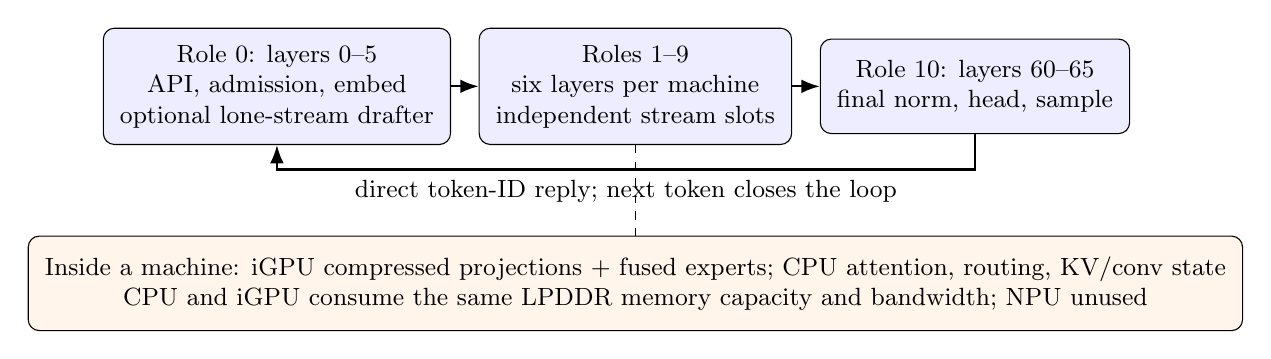
\begin{tikzpicture}[>=Latex, node distance=0.35cm, every node/.style={font=\small}, box/.style={draw,rounded corners,align=center,minimum height=1.2cm,inner sep=6pt}]
\node[box,fill=blue!7] (r0) {Role 0: layers 0--5\\API, admission, embed\\optional lone-stream drafter};
\node[box,fill=blue!7,right=of r0] (mid) {Roles 1--9\\six layers per machine\\independent stream slots};
\node[box,fill=blue!7,right=of mid] (last) {Role 10: layers 60--65\\final norm, head, sample};
\draw[->,thick] (r0) -- (mid);
\draw[->,thick] (mid) -- (last);
\draw[->,thick] (last.south) -- ++(0,-0.45) -| node[pos=.25,below]{direct token-ID reply; next token closes the loop} (r0.south);
\node[box,fill=orange!8,below=1.15cm of mid,minimum width=12cm] (devices) {Inside a machine: iGPU compressed projections + fused experts; CPU attention, routing, KV/conv state\\CPU and iGPU consume the same LPDDR memory capacity and bandwidth; NPU unused};
\draw[dashed] (mid.south) -- (devices.north);
\end{tikzpicture}}
\caption{Measured execution path. Independent streams occupy different stages concurrently. Speculative positions can overlap for a lone stream, but ordinary consecutive tokens depend on the return path. Physical box identity is separate from pipeline role.}
\label{fig:architecture}
\end{figure}

Expert weights use group-32 four-bit quantization. Attention projections and the output head use eight-bit weights. OpenVINO's fused expert path performs half-precision arithmetic; routing and sequence-state logic remain in Rust. Intended steady operation places all MoE layers on the iGPUs, but some recorded runs still contain nonfinite-output fallbacks. Thus ``iGPU-backed'' is more accurate than claiming every operation in every measured run executed on the GPU.

The all-fused configuration allocates roughly 52\,GiB of GPU page budget per machine, with a larger budget for the final role, and removes the large resident CPU expert copies. The observed ability to hold six MoE layers on a Linux rank is a fleet result. Earlier Windows single-machine notes use a different memory budget and a different paging regime; they are contextual evidence, not a matched baseline for the eleven-machine study.

\subsection{Scheduling and numerical safeguards}
The scheduler maintains stream slots and multiple frames in flight. Admission to the least populated group corrects an initial imbalance that left several groups unused. A direct final-to-first reply avoids relaying replies through every intermediate worker. Short engine steps make the submission lock available sooner, and admission can proceed while the first role waits for replies. Eight-row prefill windows subsequently allow different chunks of a prompt to occupy different stages.

For a lone request, the runtime can propose tokens from request history, a persisted phrase table, or a small external model. Verification uses the target path, and rejected predictions rewind both KV and convolution state. Multi-stream MTP execution was not deployed in the measured campaign. Gate results and numerical compatibility checks below must not be confused with preservation of the original BF16 model's output distribution.

\section{Evidence and measurement methodology}
\label{sec:method}
% Claims M01--M06.
The artifact freezes Cascadia commit \path{d1ab1abd7387b7f0b83d6d56b7aec2e1a56f9651}, with a September 21, 2026 cutoff. It covers \ExperimentCount{} experiment directories, \PhaseCount{} retained phase records and \TelemetryCount{} raw telemetry archives. Directories include proposals and interrupted work; they are not \ExperimentCount{} successful experiments. Original and scrubbed hashes are retained for \EvidenceFiles{} evidence files. Scripts reproduce tables and figures without access to the model or fleet.

\paragraph{Two throughput measures.}
For request $i$, let $n_i$ be generated tokens, $f_i$ its first-token time and $l_i$ its last-token time. The harness records
\begin{equation}
 Q_{\rm phase}=\frac{\sum_i n_i}{t_{\rm phase,end}-t_{\rm phase,start}},\qquad
 S_{\rm decode}=\sum_{i:n_i>1}\frac{n_i-1}{l_i-f_i}.
 \label{eq:metrics}
\end{equation}
$Q_{\rm phase}$ includes the admission ramp and completion tail. $S_{\rm decode}$ sums rates measured over different request intervals; it is not a synchronized steady-state token counter. Historical records call it ``steady.'' We instead use its explicit definition. The script independently recomputes every retained $Q_{\rm phase}$ from unrounded phase timestamps; all agree within the stored three-decimal rounding.

\paragraph{Token and latency semantics.}
The historical client counts nonfinal SSE events with nonempty delta objects. In the inspected sparse-MoE stream paths, including speculative emission, each generated token produces one chunk with \texttt{n\_tokens=1}; the final marker has zero tokens. Structural tokens can carry empty visible text while still having a delta object. Accordingly, counts include model tokens such as reasoning and framing tokens, and TTFT is time to the first such event, not necessarily time to the first visible answer word. The \expid{011b} server counter increases by exactly the client token count, an independent check for that run. Future harnesses should consume explicit token counts and preserve per-token timestamps rather than relying on a backend-specific chunk contract.

\paragraph{Workloads and arrival pattern.}
Requests use temperature zero and short prompts from fixed examples or deterministic family templates. Mixed phases rotate through twelve families, including explanation, code, arithmetic, story, rewriting and translation. The default ``burst'' launch staggers requests by 15\,ms; explicitly staggered phases use approximately one second. Prompts labeled fresh are generated from experiment tags, so most before/after phases are not identical-prompt pairs. Repeated prompts train the persisted phrase proposer. We expose output caps, concurrency, completion counts and prompt-history limitations alongside results.

\paragraph{Correctness checks.}
The serial gate compares three 32-token references, but its acceptance predicate is weaker than full equality: it requires nonbroken outputs and sufficient matching prefixes on at least two prompts. The concurrent gate also checks prefixes. Selected configurations answer twelve simple known-answer questions correctly; these are smoke tests, not a benchmark of general capability. Several half-precision runs diverge from a reference after a shared prefix. Throughout this paper, a gate pass means that check passed, not that all outputs are bit-identical or that quantization is quality-neutral.

\paragraph{Telemetry and uncertainty.}
Profiles report computation, projection, expert, head and wait times. Repeated relay records are deduplicated and assigned to the operator clock using receipt age; installed-box and pipeline-role identifiers remain separate. This repairs a known final-rank clock jump. Per-frame timings are averages over retained decode windows, not hardware performance-counter measurements. Most configurations have one or two phase runs, accumulated during an exploratory campaign with evolving software and thermal state. We report observations without inventing confidence intervals or treating thousands of correlated token positions as independent replicates. Five incomplete or failed phase records are retained and excluded from headline success claims.

\section{Measured service behavior}
\label{sec:service}

\subsection{Capacity and high-concurrency throughput}
% Claims P01--P03.
The model is served by the whole fleet, not replicated eleven times. Table~\ref{tab:throughput} follows the principal 176-stream configurations. The progression moves from CPU experts to partial and then full iGPU expert execution, moves dense blocks to the iGPU, and parallelizes the CPU attention work across independent rows. Configuration changes are cumulative and sometimes bundled, so the sequence does not identify the isolated causal contribution of each feature.

\begin{table}[ht]
\centering\small
\begin{tabular}{llrrrr}
\toprule
Exp. & Configuration & Cap & Completed & $Q_{\rm phase}$ & $S_{\rm decode}$\\
\midrule
005 & CPU experts; short engine steps & 48 & 176/176 & 19.414 & 29.566\\
007 & Partial fused iGPU experts & 32 & 176/176 & 26.839 & 44.624\\
008b & All MoE layers on iGPU path & 32 & 176/176 & 32.651 & 55.609\\
009 & Dense blocks also on iGPU & 32 & 176/176 & 34.847 & 57.917\\
011 & Parallel attention over rows & 32 & 176/176 & 37.024 & 64.175\\
011b & Same family, longer generations & 128 & 176/176 & \LongPhaseRate & \LongSumRate\\
\bottomrule
\end{tabular}
\caption{Observed 176-stream throughput in generated tokens/s. Cap is requested maximum output tokens per stream; early stopping can reduce total output. The first row uses a different cap, and the final row measures a longer phase. No controlled fleet-scaling multiplier is inferred.}
\label{tab:throughput}
\end{table}

\begin{figure}[ht]
\centering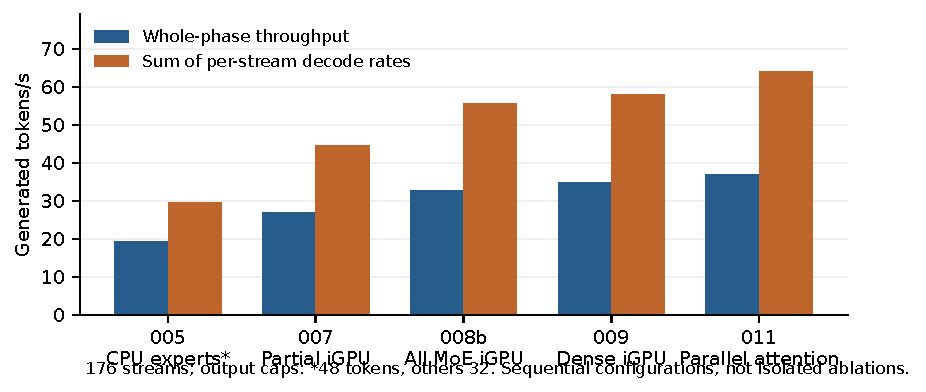
\includegraphics[width=\linewidth]{figures/throughput.pdf}
\caption{The two throughput definitions differ materially during admission-heavy phases. Values are regenerated from retained phase JSON rather than copied from the leaderboard.}
\end{figure}

In \expid{011b}, all 176 requests complete, generating \LongTokens{} tokens over \LongSeconds{} seconds. Mean TTFT is \LongTTFT{}\,s. Raw server counters independently record the same token total. Figure~\ref{fig:counter} shows why the whole-phase rate remains below the decode plateau. In a separate audit calculation, disjoint blocks of five roughly two-second polls, selected when both endpoints have at least 170 requests in flight, have median \CounterMedian{} tokens/s but mean \CounterMean{}. The subset still contains prefill ramp-up: requests in flight are not synonymous with requests decoding. The historical 70.5-token/s server median used another sampling alignment; we do not present either selection as a replicated benchmark.

\begin{figure}[ht]
\centering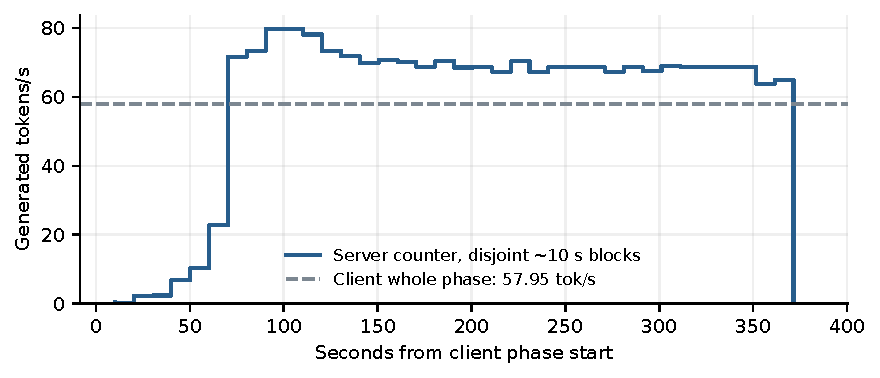
\includegraphics[width=\linewidth]{figures/counter.pdf}
\caption{Independent server token-counter reconstruction for \expid{011b}. The trace includes admission, the decode plateau and the completion tail. Bins are disjoint five-poll intervals anchored at the first retained poll.}
\label{fig:counter}
\end{figure}

Additional concurrency is not a free improvement. A complete 352-stream run in \expid{009} records 54.9 summed decode tokens/s, below its 176-stream result, with substantial memory pressure. Earlier 264- and 352-request attempts lose client connections and are explicitly excluded as successful full-concurrency runs. These observations demonstrate the configuration's limits; they are not a general statement about the GPU's maximum serving concurrency.

\subsection{Fifteen streams and time to first token}
% Claims P04--P06.
At fifteen streams, \expid{019} records summed decode rates of 22.544 and 23.383 tokens/s, whole-phase rates of 15.678 and 17.005, and median TTFTs of 31.52 and 31.23\,s. Each phase requests 128 output tokens per stream. With eight-row prefill windows, \expid{024}'s corresponding burst completes at 22.521 whole-phase tokens/s and 24.626 summed decode tokens/s, with median TTFT 6.91\,s and maximum 10.03\,s. This is an observed approximately 4.5-fold reduction in median TTFT across these phases, not a randomized same-prompt estimate.

One-second arrival staggering in \expid{024} produces median TTFT 2.48\,s, and two isolated requests record 1.96 and 2.11\,s. Later fifteen-stream configurations generally remain around 24--25 summed decode tokens/s. In \expid{027}, the two per-stream median decode rates are 1.654 and 1.636 tokens/s, so fleet aggregate throughput should not be mistaken for fast individual conversation. The fifteen-stream target of 60 tokens/s was not achieved.

\begin{figure}[ht]
\centering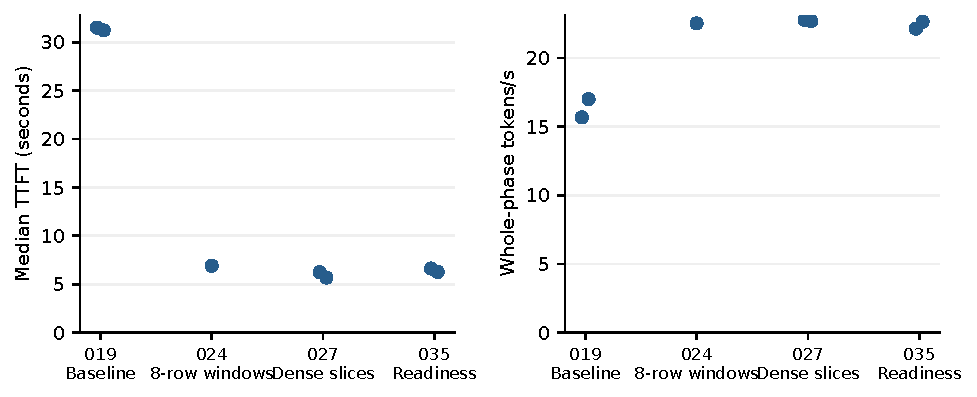
\includegraphics[width=\linewidth]{figures/prefill.pdf}
\caption{Recorded burst-phase medians and whole-phase throughput at fifteen streams. Each dot is one phase, not a confidence interval. Tags and software differ across experiments; \expid{035} adds readiness protection, not a claimed throughput gain.}
\label{fig:prefill}
\end{figure}

\subsection{Single-stream speed depends on the text}
The ensemble proposer in \expid{015c} yields approximately 3.1--3.4 tokens/s on explanation prompts, 3.38 on a story, 3.67 on code, 5.85 on rewriting, 6.60 on translation, 8.19 on arithmetic and 10.95 on a true/false prompt. These are small task-conditioned samples, not task-wide means. They mix accepted history proposals and small-model proposals; some prompt families were previously observed during collection.

Transferring retained phrase history in \expid{038} improves several repeated requests, including code from 5.225 to 10.600 tokens/s. The baseline requests themselves update the table and the release changes capture behavior. This validates retained-history functionality but does not isolate the merge's causal effect or establish an unseen-prompt improvement. We exclude these repeated-prompt rates from general single-stream capability claims.

\section{Local improvements and closed-pipeline limits}
\label{sec:limits}

\subsection{A dense block through a fused expert operator}
% Claims K01--K03.
A dense SwiGLU block can be partitioned along its intermediate dimension:
\begin{equation}
 W_d[\operatorname{SiLU}(W_gx)\odot W_ux]
 =\sum_{j=1}^{8}W_{d,j}[\operatorname{SiLU}(W_{g,j}x)\odot W_{u,j}x].
 \label{eq:dense}
\end{equation}
All slices remain active with unit routing weights. The algebra is established, including especially close prior work in MLPMoE~\cite{mlpmoe} and broader dense-to-expert work in MoEfication~\cite{moefication}. Cascadia uses it to access a favorable compressed fused-expert implementation for the two dense layers.

Experiment \expid{027} measures approximately 8.1\,ms per dense layer with three compressed matrix operations versus 4.5\,ms through eight fused slices. The two FP16 paths differ by relative error $5.7$--$5.9\times10^{-4}$ in the retained load checks; the real-arithmetic identity does not imply bitwise identity after regrouping finite-precision operations. Role 0's measured computation falls from 51.9 to 43.7\,ms per frame. The mean summed fifteen-stream decode rate rises only from 24.6355 to 24.790, approximately 0.63\%. The comparison still includes the earlier group-64 canary, so it is not the final unchanged-weight serving baseline. The local improvement shifts which stage matters without proportionately accelerating the fleet.

\subsection{Sharing output-head calls saves work but delays replies}
% Claims K04--K05.
In \expid{028}, the last stage combines output-head work for waiting frames. Across the two fifteen-stream phases, $S_{\rm decode}$ falls from mean 24.790 in \expid{027} to 24.119, a \HeadRegression\% regression. The archived verdict rounds this differently. Corrected decode-window telemetry for phase A reports head time falling from 11.62 to 7.32\,ms per frame, while computation remains about 36 and 35\,ms respectively. Figure~\ref{fig:head} makes the mismatch between local work reduction and service throughput explicit.

\begin{figure}[ht]
\centering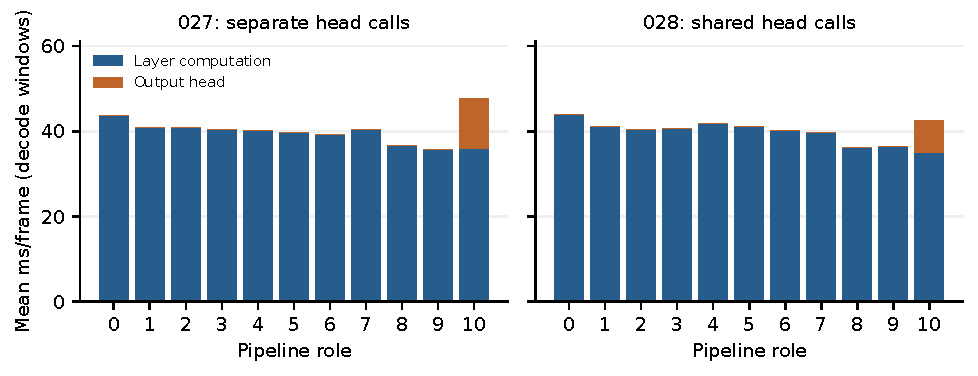
\includegraphics[width=\linewidth]{figures/head_batching.pdf}
\caption{Reconstructed role profiles after deduplication and clock alignment. Output-head work decreases under batching, yet summed decode rates regress. These bars omit communication and waiting and should not be read as full request latency.}
\label{fig:head}
\end{figure}

An autoregressive request cannot create its next frame until its current token returns. Delaying a reply can remove useful work from other stages even if it reduces output-head traffic. At fifteen streams in eleven groups, frames also alternate between one and two rows. FIFO queueing behind longer frames can produce convoy effects. These mechanisms are consistent with the observed regression, but the experiment does not uniquely identify their individual contributions. In particular, it also removes the previous group-64 canary, and prompt tags differ. We report the observation and a scheduling explanation, not a universal prohibition on head batching.

\subsection{A useful model, and an explicit failed prediction}
% Claims B01--B04.
For small frames, the journal's empirical stage approximation is
\begin{equation}
 t(r)\simeq16+19r\quad\text{milliseconds},\qquad 1\lesssim r\lesssim3.
 \label{eq:stage}
\end{equation}
It summarizes fixed per-frame projection and operator costs plus row-dependent expert and CPU work on the constrained middle stages. It is neither a fitted universal hardware law nor a model of large batches. For $C$ streams in $F$ equal-sized frames across $D$ stages, an idealized cycle-time lower bound is
\begin{equation}
 T_{\rm cycle}\geq\max\left(\sum_{j=1}^{D}t_j(C/F),\; F\max_jt_j(C/F)\right).
 \label{eq:cycle}
\end{equation}
The first term expresses one frame's sequential traversal; the second expresses the busiest stage's work per cycle. Unequal frame sizes, communication, admission and scheduling add delay. We use this classical service-demand reasoning to organize evidence, not as a new queueing theorem.

A journal calculation predicted that reducing $F$ from eleven to ten would improve fifteen-stream service. Experiment \expid{034} uses the same prompt tag, phase names and binary and falsifies that prediction: the two phases change from 24.580/24.679 to 24.596/24.444 summed tokens/s. At 176 streams the change is 67.974 to 64.846, a \InflightRegression\% regression. Eleven frames are restored. The model identifies relevant terms but does not resolve scheduling interactions well enough to optimize frame count without measurement.

\subsection{Memory-traffic estimates are conditional bounds}
The export-size accounting in the lab notes estimates about 16.76\,GB of active expert weights, 8.59\,GB of attention projections, 0.52\,GB of dense weights and 1.24\,GB of output-head weights for one unshared full-model token: approximately 27.1\,GB. Quantization scales and zero points are included in the expert estimate. These are logical weight bytes, not measured DRAM transactions; caches, reuse and extra reads can change physical traffic. This is the distinction required by bandwidth-oriented performance modeling~\cite{roofline}.

A pipeline token visits the layer partitions sequentially. Even though eleven memory buses exist, a single ordinary token cannot read every layer on all buses at once. Concurrent requests fill the pipeline; speculative positions provide another opportunity to overlap work, at the cost of rejected computation.

Using the notes' approximate layout, a six-MoE-layer stage at $C=15,F=11$ accounts for $11(0.78)+15(1.57)\simeq32.1$\,GB of logical weight reads per cycle. The final stage additionally applies an approximately 1.236\,GB head per frame, increasing this estimate to about 45.7\,GB. Omitting the head underestimates that stage's service demand. Under the explicit assumptions of no inter-frame weight reuse, one head read per frame and 136.5\,GB/s sustained bandwidth, its byte-only ceiling would be roughly 45 tokens/s, before CPU work and other overheads. The 136.5 value itself assumes 8533\,MT/s on a 128-bit interface; it is not an independently measured fleet-wide sustained bandwidth. We therefore do not claim a topology-independent physical impossibility of 60 tokens/s. We conclude that the measured configuration is well short of that target and that improving it requires changing service demand or scheduling, not merely increasing nominal concurrency.

The notes' earlier characterization of 60--65\,GB/s as the memory-bus limit was also too strong. It described a particular CPU expert path. The output head moves logical weight bytes at approximately 108\,GB/s by byte/time accounting. The fact that one kernel reaches that rate does not prove every other kernel can reach it, but it disproves treating a slower kernel's effective rate as the platform's peak bandwidth.

\section{Failure analysis and negative experiments}
\label{sec:failures}

\subsection{Fallback can destroy unified-memory residency}
% Claims F01--F03.
An iGPU allocation and a CPU expert cache consume the same physical memory. In \expid{007}, nonfinite results on one layer trigger CPU fallbacks and an additional expert cache, leaving very little memory on the affected machine. Attenuating the relevant up-projection scales and restoring output scale permits subsequent all-fused operation, but does not establish general equivalence to the original high-precision model.

Experiments \expid{021} and \expid{022} initially appear to show a GPU-kernel crash. Later journal evidence in \expid{025} identifies a different chain: a failed GPU inference call, repeated CPU fallback, duplicate expert residency, swap exhaustion and an operating-system OOM kill. The lower-level source investigation also identifies a group-size/subgroup compatibility restriction. A patch that enables group-32 execution passes the retained load checks in \expid{029}, but one-row calls still take approximately 3.0--3.2\,ms. Correcting compatibility does not itself accelerate the operator.

This supports a specific design lesson: fallback must be budgeted together with the allocations that remain alive. A fallback that preserves a numerical result can still remove the memory headroom needed to keep a pipeline resident. The study does not establish that the identified restriction remains present in newer OpenVINO versions; the evidence is tied to the recorded 2026.3.1 plugin hash.

\subsection{Several plausible sources of idle time did not pay}
% Claims N01--N04.
\begin{table}[ht]
\centering\small
\begin{tabularx}{\linewidth}{lXX}
\toprule
Experiment & Hypothesis or intervention & Observed limit\\
\midrule
020 & Reuse projection input tensors & No material improvement in the recorded comparison; attention profiling shows substantial device execution.\\
023 & Overlap GPU calls with two stage threads & Approximately 1.04--1.10$\times$ device-call improvement, below the predeclared 1.25$\times$ threshold.\\
026, 029 & Use MoE-specific decode kernels & Group-64 changes weights; group-32 compatibility patch is not faster at one row.\\
029 & Sleep while waiting for GPU completion & Lower busy CPU usage and package power, but about 2.3\,ms more per frame on the canary role.\\
034 & Reduce circulating frames to ten & Fifteen-stream rates essentially unchanged; 176-stream rate regresses.\\
\bottomrule
\end{tabularx}
\caption{Negative results delimit the tested implementations. They do not prove that overlap, specialized kernels or power-aware waits can never help on other workloads. Per-role comparisons also contain layer and device differences.}
\end{table}

\subsection{Network behavior depends on the communication pattern}
% Claims N05--N06.
Disabling the documented USB NCM aggregation timer~\cite{cdc} reduces reported small-payload round-trip latency from about 3.3\,ms to 0.2--0.3\,ms when both endpoints are configured; 12\,kB probes remain slower. This is an application of an existing driver control. It is not proof that the complete inference round trip improves by the same factor.

The separate all-to-all probe in \expid{018} uses 100\,kB request/reply messages with the model idle. At a target of 30\,MB/s per box, all eleven participate; at 50\,MB/s, achieved rates plateau around 41--45\,MB/s and high-percentile delays increase. Earlier low-rate steps have only a subset of machines and must not be labeled eleven-node tests. The rank grouping of losses is consistent with a shared bottleneck between switch groups, but the physical wiring was not verified. Nor was full-model expert-parallel inference measured on this fleet: a communication probe is not an expert-parallel serving result.

\subsection{Role relocation and readiness are operational results}
Experiment \expid{032} moves logical roles while preserving installed-box identity and the existing ingress relay. It reduces role 0's stage time, but leaves the suspect entry machine and its relay responsibilities in the deployment. Subsequent short successful load tests do not establish a hardware repair or sustained availability. Experiment \expid{035} adds a stateless full-chain readiness probe before request admission; the retained integration-test account exercises delayed startup without generation traffic. Neither result warrants importing the architecture paper's broad node-loss or decentralized-availability claims into this eleven-stage chain.

\section{Draft-head qualification on the deployed numerical path}
\label{sec:mtp}
% Claims D01--D06.
Speculative decoding and learned feature proposals are established techniques~\cite{specdecode,eagle}, as is multi-token prediction~\cite{mtp}. The question here is whether Inkling's shipped head is useful for this particular quantized fleet and its available stage slack.

Experiment \expid{033} evaluates eight chained MTP modules on 36 CPU-reference sequences: three prompts from each of twelve families, with 160 generated positions per sequence. First-draft agreement is reported as 0.726. The CPU-generated text diverges from the fleet path, so \expid{039} repeats qualification on captured fleet states and actual emitted token IDs. The table below reports offline agreement, not live speculative acceptance or runtime speed.

\begin{table}[ht]
\centering\small
\begin{tabular}{lr}
\toprule
Calculation & First-draft agreement\\
\midrule
CPU-reference sequences, original head (033, rounded) & 72.6\%\\
Fleet sequences, original head (039) & \MTPFleet\%\\
Fleet sequences, original head restricted to 65,536 tokens & 64.54\%\\
Fleet sequences, INT4/INT8 weights and 65k head & \MTPDeployment\%\\
\bottomrule
\end{tabular}
\caption{The fleet rescore uses 5,724 first-draft targets from 36 sequences. The CPU-to-fleet difference combines trajectory and numerical-path changes and is not an isolated quantization ablation. The deployment-grid calculation uses FP32 arithmetic, not actual GPU execution.}
\label{tab:mtp}
\end{table}

The original and deployment-grid fleet agreements both miss the study's 0.70 qualification bar. On the same fleet states, restricting the original vocabulary accounts for most of the subsequent decrease; additional quantization contributes approximately 0.175 percentage points. The deployed-grid agreement varies by family, including about 0.482 for story, 0.746 for code and 0.748 for arithmetic. Only three sequences represent each family, so these are descriptive slices.

\begin{figure}[ht]
\centering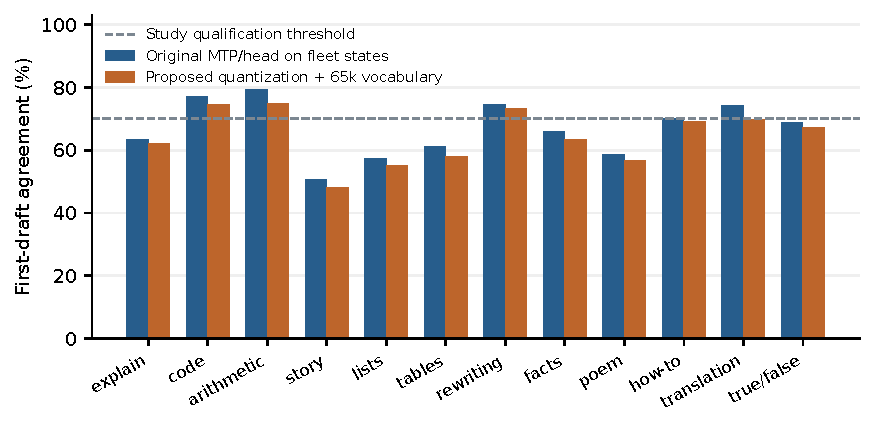
\includegraphics[width=\linewidth]{figures/mtp.pdf}
\caption{First-draft agreement on fleet sequences, regenerated from \expid{039}. No bars represent live serving speed. The qualification threshold is a study decision, not a universal break-even acceptance rate.}
\end{figure}

Temporal state matters as well as first-draft accuracy. Each chained module has its own attention and convolution history. In the fleet rescore, expected accepted drafts across eight modules are reported as 2.128 with teacher context, 2.007 with self-fed context, and 0.769 without deeper-module context. A single exported module cannot inherit an eight-module projection. MoESD and more recent MoE-specific speculative systems already show that verification cost and expert activation affect benefit~\cite{moesd,moespec,specmoe}; this experiment adds deployment-specific evidence, not a new general principle.

Capturing states exposes another numerical boundary. The first FP16 capture format overflows; a sampled pre-final-normalization residual reaches magnitude 4,272,968. The corrected format stores FP32 residuals. All 36 captured responses pass the retained finite-value and API-text checks before rescoring. Reapplying the original BF16 output head agrees with actual fleet token IDs at only 92.12\% of positions, further motivating use of emitted IDs as the target. That agreement is not a general quality score.

Finally, intermediate-boundary vocabulary probes in \expid{033} do not qualify as drafters under the study's cost model. Raw top-one agreement rounds to zero through the first five boundaries; affine probes improve it but remain below the stated break-even bars. This is a negative result for the evaluated protocol, not a claim that intermediate states contain no predictive information or a replacement for tuned-lens research~\cite{tunedlens}.

\section{Related work and scope of novelty}
\label{sec:related}
Petals, TPI-LLM, prima.cpp and exo establish distributed inference on consumer or edge devices~\cite{petals,tpi,prima,exo}. The existing Cascadia shard paper establishes this project's Intel/OpenVINO pipeline and speculation lineage~\cite{shards}. Our fixed resident MoE fleet supplies a different model and hardware operating point; pipeline partitioning itself is not new.

EdgeMoE and PowerInfer address memory and sparsity on resource-constrained hardware~\cite{edgemoe,powerinfer}. Klotski studies expert-aware multi-batch scheduling, MegaScale-Infer disaggregates attention and expert work, and EC2MoE studies edge/cloud pipeline collaboration~\cite{klotski,megascale,ec2moe}. Contemporary CPU/discrete-GPU hybrid work also measures prefill, concurrency and overlap~\cite{hybrid2026}. These systems rule out broad claims to have discovered that MoE serving is memory-sensitive or that expert placement must account for communication.

Orca and SARATHI/Sarathi-Serve provide the scheduling context~\cite{orca,sarathi,sarathiserve}: iteration-level admission, prefill chunking and pipeline balance are established. Likewise, the dense-block decomposition in Equation~\ref{eq:dense} has close prior art~\cite{moefication,mlpmoe}. The evidence supports a measured compiler-path optimization, not a new transformation.

The closest same-model deployment lead is the August 2026 first-person report of Inkling-NVFP4 on eight DGX Sparks~\cite{sparkinkling}. It uses larger memory per device, a different interconnect, tensor parallelism, another numerical format and MTP. Its reported performance is neither a matched baseline nor independently reproduced here. It nevertheless makes a broad ``first small cluster running Inkling'' claim untenable.

The defensible novelty is therefore empirical and integrative: the residency and fallback behavior of a nearly trillion-parameter sparse model on this integrated-GPU fleet; the measured disconnect between per-stage work reduction and closed-loop service improvement; and the qualification gap between CPU-reference and actual deployed-path drafting. We describe these as candidate systems findings supported by a bounded literature search through September 21, 2026. Search absence cannot establish absolute priority.

\section{Limitations and next measurements}
\label{sec:limitations}
The campaign is a single deployment, with short synthetic prompts, evolving software, thermal and power heterogeneity, and limited independent repetition. Prefix gates and simple question checks do not establish full model quality. The artifact does not provide every original weight manifest, GPU driver/firmware identifier or MTP tensor capture, and does not support complete end-to-end reproduction from the repository alone. It does support regeneration and inspection of the reported measurements.

The most useful next experiment is a frozen, randomized A/B repetition of the fifteen-stream baseline, prefill windows and head batching with identical prompts, a controlled proposer history, full token-ID traces, and TTFT/inter-token-latency distributions. A separate evaluation should compare the deployed numerical path to the original model on a held-out quality corpus and longer contexts. Complete per-box hardware, driver and memory-timing inventories and wall-power measurements would enable reliable efficiency analysis. Such measurements were not run for this retrospective paper preparation.

INT4 attention is only a microbenchmark result: \expid{041} reports 39.0--43.2\% shorter projection calls on two layers at one or two rows, with approximately 9.6--9.7\% relative RMS output difference on random inputs. No end-to-end fleet gain or model-quality outcome is established. The expert-usage collection in \expid{040} is interrupted, and fleet-trained drafting, an INT4 serving canary, CPU/GPU overlap and full expert-parallel serving remain proposals or unfinished work at the cutoff. They do not appear as achieved capabilities.

The dataset does not establish purchase cost, energy per token, million-token context, multimodal support, sustained availability, or superiority to datacenter hardware. All power numbers refer to telemetry domains, and all comparisons across hardware would require matched workloads and numerical formats.

\section{Conclusion}
Eleven 64\,GB Panther Lake machines can supply the memory and execution resources to serve Inkling's large text decoder. The measured result depends strongly on concurrency and metric: \LongPhaseRate{} tokens/s over a complete 176-request phase, versus roughly 22--23 whole-phase tokens/s in the improved fifteen-request phases and much lower individual stream rates. The study's reusable findings concern how unified-memory residency, operator dispatch, numerical range, return-path scheduling and deployment-specific draft qualification interact. Retaining failed hypotheses and reconstructing the measurements narrows the claims while making the system easier to understand and reproduce.

\paragraph{Artifact availability.}
Paper source, derived tables, scrubbed telemetry, evidence hashes and offline reconstruction scripts are maintained at \url{https://github.com/labscommunity/cascadia-inkling-panther-lake-paper}. The repository is private during author review. \path{reproduction/CLAIMS.md} maps quantitative statements to evidence; \path{reproduction/AUDIT.md} records corrections and limitations; \path{research/NOVELTY.md} records prior-art judgments. Public artifact availability is pending an author-controlled release.

\bibliographystyle{plainnat}
\bibliography{references}
\end{document}
